% This is a template for the assignment reports
% TARI29 Artificial Intelligence, 7.5 credits, Winter 2024
% Original version by:  Vladimir Tarasov, 2024
% Revised by:           Alexandros Tzanetos, 2024 

% Use a modern class instead of an old article class
\documentclass{scrartcl}

\KOMAoptions{
    parskip=half,  % full, off
    fontsize=12pt, % base font size (10pt default)
    % headings=big,% small/normal/big headings (normal is default), 
    % paper=a5,    % paper format (a4 default) 
    pagesize=auto  % Use paper format for PDF too
}

% ---------------------- Report details --------------------- %
\newcommand{\docauthor}{Ben Bekir Ertugrul, Moritz Schlitter}
\newcommand{\courseyear}{2026}
\newcommand{\coursename}{TDIS22 Deep Learning}
\newcommand{\coursecredits}{7.5 credits}
\newcommand{\fullcoursename}{\coursename, \coursecredits}
\newcommand{\termname}{Spring \courseyear}
\newcommand{\groupnumber}{MS BE}
\newcommand{\reportname}{Assignment 2 Report: English to Spanish Translation}
\newcommand{\assignmentname}{Assignment Group \groupnumber\ Report}
% ------------------ End of report details ------------------ %



% ---------- Setting up properties of the PDF file ---------- %
\usepackage{hyperref}
\hypersetup{
    colorlinks=true,
    allcolors=blue,
    pdftitle={\reportname},
    pdfauthor={Name1, Name2},
    pdfsubject={\coursename, \termname}
	% pdfpagemode=FullScreen,
	% pdfpagemode= UseOutlines % the default if present
}
% ------------ End of properties of the PDF file ------------ %



% ----------- Setting up the headers and footers ------------ %
\usepackage{scrlayer-scrpage}
\pagestyle{scrheadings}
\KOMAoptions{% 
    headsepline,% line below the header
    plainheadsepline,% also on scrplain
}
\clearscrheadfoot % Erase all current configurations
% inner part of the header [titel_page]{other_pages}
\ihead[\coursename, \courseyear]{\coursename, \courseyear}
% outer part of the header [titel_page]{other_pages}
\ohead{\assignmentname}
% center part of the footer [titel_page]{other_pages}
\cfoot[\textup{Page \pagemark\ of \ztotpages}]{\textup{Page \pagemark\ of \ztotpages}}
% ------------- End of the headers and footers -------------- %



% ---------------- Setting up the title page ---------------- %
\title{\reportname}
\subtitle{\assignmentname}
%\author{\docauthor}
\author{Ben Bekir Ertugrul \and Moritz Schlitter
}
\date{\today}
% ------------------ End of the title page ------------------ %

\usepackage[english]{babel}

% --------------- Packages and custom commands -------------- %
% Specify the input encoding of the source file as UTF8 
\usepackage[utf8]{inputenc}
% The T1 font encoding is an 8-bit encoding and fully supports words containing accented characters
\usepackage[T1]{fontenc}
% Load Latin modern fonts in outline format
\usepackage{lmodern}
% Load better typewriter font
\usepackage{inconsolata}
% For better hyphenation patterns
\usepackage[english]{babel}
% For improved micro-typography
\usepackage{microtype}
% Switch off extra space after a sentence
\frenchspacing
% To be able to iclude pictures
\usepackage{graphicx}
\usepackage{adjustbox}
\usepackage{subcaption}
\usepackage{zref-totpages} % To get the total number of pages
\usepackage{mathtools,amsmath} % for advanced math formulas
 % To highlight source code
\usepackage{minted}
% Default options for all minted environments
\setminted{
           style=default, % for minted envronment
           autogobble, % automatically remove all common leading whitespace
           xleftmargin=10pt, % indentation to add (on the left) before the listing
           numbersep=6pt, % gap between numbers and start of line
           linenos, % enables line numbers
           mathescape % enables the usual math mode inside comments
}
\setmintedinline[c]{style=default} % for minted inlines
% Flexible handling of verbatim text
\usepackage{fancyvrb}
% For well-spaced lines and guidelines in tables
\usepackage{booktabs}
% To typeset algorithms or pseudocode in LaTeX 
\usepackage{algorithm}
\usepackage{algpseudocode}
% For plots and graphs
\usepackage{pgfplots}
\pgfplotsset{width=10cm,compat=1.9}
% for quotes " " with \enquote{text}
\usepackage{csquotes}
% for \begin{enumerate}[resume] to work. resumes counting instead of starting from 1 again.
\usepackage{enumitem}

% To generate placeholder text - can be deleted when you have written real text
\usepackage{lipsum}
% ----------- End of packages and custom commands ----------- %

\begin{document}

\maketitle

% It can be commented out if you do not want the table of contents
\pagebreak
% \tableofcontents
% \pagebreak

% \include{introduction}
% \include{preprocessing}
% \include{models}
% %\include{results}

% \bibliographystyle{ieeetr}
% %\bibliography{references}

% \appendix 
% \include{appendix}
\section{Results}

\begin{figure}[htbp]
\centerline{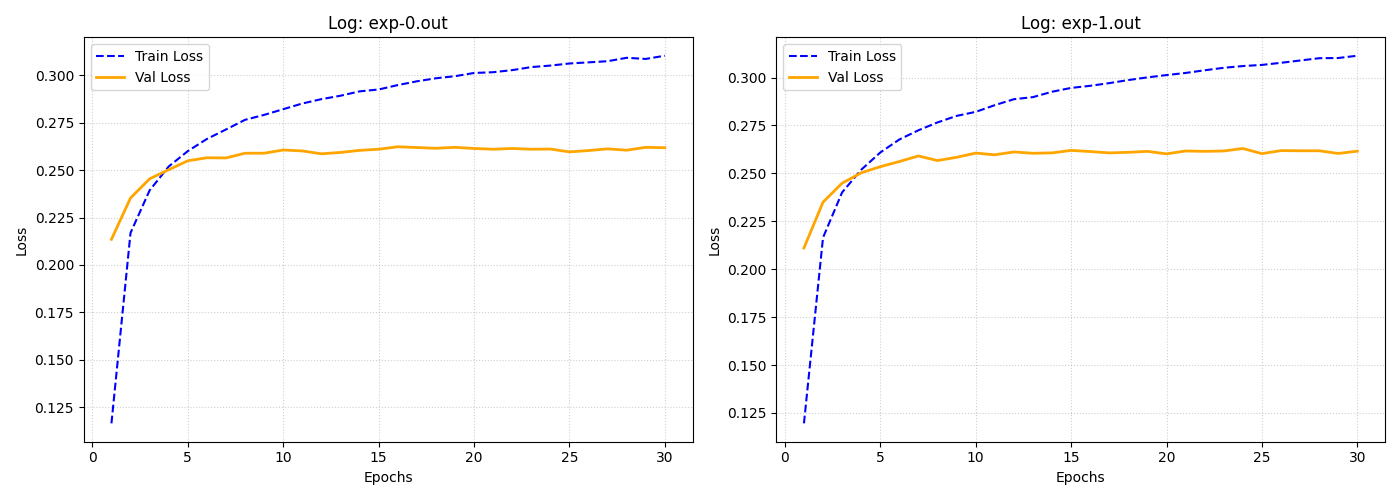
\includegraphics[width=\columnwidth]{resources/logs.png}}
\caption{Training and validation accuracies for experiment 0 and 1 over the duration of the training process.}
\label{fig:results}
\end{figure}

\subsection{Experiment 0}
Experiment 0 concerns itself with the training of a transformer model for the task of english to spanish translation. This sets a baseline performance for the following experiment, which implements a custom multi-head-attention layer.

The training process of this experiment is shown in figure \ref{fig:results} on the left. In epoch 1, the model achieves a training accuracy of about 0.1165. The accuracy slowly improves until the epoch 30, where it ends up at 0.3103. The validation accuracy starts at 0.21, reaches 0.2589 in epoch 8, and then stagnates. The highest validation accuracy is reached in epoch 16 with a value of 0.2623.

\subsection{Experiment 1}
The model for experiment 2 is built on a custom multi-head-attention layer which is used only for the encoder step inside the transformer. The rest of the architecture is identical to that of experiment 0.

Figure \ref{fig:results} shows the output of experiment 1 in the right corner. Being trained for 30 epochs in total, the training accuracy was increased from 0.1196 to 0.3114. The validation accuracy starts off with 0.2111 in the first epoch. Similar to experiment 0, we can see it reaching 0.2591 in epoch 7 and then stopping to improve. The final validation accuracy is 0.2616.

\subsection{Experiment 2}
todo

\section{Discussion}
The goal of this was to show performance differences between the usage of official and custom multi-head-attention layers.

However, we can see that there is almost no difference. The custom implementation performs slightly better for this training run, but that could be the result of a lucky random intialization for the $W^q$, $W^k$, $W^v$, and $W^o$ matrices.
Moreover, measuring the total time of the training process, we saw that experiment 0 took 1515.8 seconds, while experiment 1 took only 1355.2 seconds.

One of the reasons why our implementation is able to keep with the official implementation, is that we make use of similar optimizations. When using $N$ attention heads, we do not keep $N$ sets of matrices and do not perform our computation $N$ times in total. Instead, we work with one regular set of matrices, as used for single-head-attention, and reshape them before applying the Softmax, so that they act as individual attention heads.

\section{Conclusion}
todo
\end{document}
